\documentclass[twocolumn, 10.5pt]{article}
\usepackage{verbatim}
\usepackage{amsfonts}
\usepackage{geometry}
\usepackage{amsmath}
\usepackage{amsthm}
\usepackage{amssymb}
\usepackage{listings}
\usepackage{graphicx}
\usepackage{clrscode3e}
\usepackage{txfonts}
\usepackage{fontspec}
\usepackage{float}
\usepackage{enumerate}
\setmainfont{Times New Roman}
\geometry{top=2.5cm,bottom=2.5cm,left=2.5cm,right=2.5cm}
\setlength\parindent{0em}
\begin{document}
	\title{Problem Solving Homework (Week 2)}\author{161180162 Xu Zhiming}\maketitle
	\section*{TC Chapter 34}
	\subsection*{34.1-2}
	The formal definition:\\
	Input: Instance of some undirected graph\\
	Output: A simple cycle\\
	Relation between them: The instance graph contains the cycle, and such cycle is of the largest length.\\
	The decision problem is: \proc{Longest-Cycle}=$\{\left\langle G,u,k\right\rangle:\ G=(V,E)$ is an undirected graph, $u\in V,\ k\le 0$ is an integer, and $G$ contains a simple cycle starting from $u$, which has at most $k$ edges$\}$.\\
	The language is the same as \proc{Longest-Cycle}
	\subsection*{34.1-3}
	Suppose the alphabet is $\{0,1,\#,*\}$, where $\#$ represents another column and $*$ denotes another row. Then the adjacent matrix representation of a directed graph is as follows ($BiStr[i]\in\{0,1\}^*$ is the distance between $\lfloor i/n+1\rfloor$ and $\lceil i\%n\rceil$):
	\[
	\begin{aligned}
	BiStr[0]\#BiStr[1]&\#\cdots BiStr[n-1]*\\
	BiStr[n]\#BiStr[n+1]&\#\cdots BiStr[2n-1]*\\
	\cdots&\cdots\\
	BiStr[n^2-n]\#BiStr[n^2-n+1]&\#\cdots BiStr[n^2-1]*\\
	\end{aligned}
	\]
	The adjacent table is:
	\[
	\begin{aligned}
	(s_1[0],s_2[1])(s_1[2],s_2[3])&\cdots (s_1[m],s_2[m])*\\
	\cdots&\cdots\\
	(s_1[l],s_2[l])(s_1[l+1],s_2[l+1])&\cdots (s_1[l+m],s_2[l+m])*
	\end{aligned}
	\]
	$s_1$ denotes the to which vertex, and $s_2$ denotes the length of such edge.\\
	Obviously, we can think of the adjacent table as a partially-filled adjacent matrix, with empty entries implying no existence of edges. Since the matrix is of $O(n)$ size, we can fill the blanks in $O(n)$ time, yielding the correspondent matrix. Vice versa, remove the $BiStr$ that equals $0$ produces the adjacent matrix. Therefore, the two forms are polynomially related.  
	\subsection*{34.1-5}
	\begin{proof}
		Suppose the running time of such polynomial algorithm is $O(n^{c_1})$, where $n$ is the input size and $c_1$ is some constant. The subroutine's running time is $O(n^{c_2})$ (Symbols' meanings are alike). Consider the following situations.
		\begin{itemize}
			\item Call the subroutine for constant times $c_3$: The running time of such subroutine is bound in $c_3\cdot O(n^{c_2})$. Literally, it is $O(n^{c_2})$ as $c_3=O(1)$, thus making almost no difference to the overall time complexity $O(n^{c_1})$. Therefore, it remains a polynomial-time algorithm.
			\item Call the subroutine for polynomial times $O(n^{c_4})$:  If the polynomial's degree is relevant to the input size $n$, for example, square the input $x$. Then subroutine of doing product runs for $$x^{2^{\log_2 x}}=x^x=2^{x\log_2 x}=2^{\log_2 x{\log_2 x}}=O(2^x).$$
			It is of exponential time complexity.
		\end{itemize}
	\end{proof}
	\subsection*{34.2-3}
	\begin{proof}
		Since $\proc{Ham-Cycle}\in \text{P}$, the following procedure can help us determine the vertexes in order, and it is still in P. Suppose the algorithm is named \proc{Ham-Solver$(G)$}, and it returns \emph{true} if $G$ has a Hamilton cycle, \emph{false} if not. 
		\begin{codebox}
			\zi
			\proc{Vertex-In-Ham-Cycle$(G)$}\li
			Initialize an empty  edge set $V_H$\li
			\If $\proc{Ham-Solver(G)}==\const{false}$\li
			\Do \Return \const{null}\End \li
			\Else\li\Do  
			\For edges  $(u,v)$ in $G.E$\li
			\Do Remove the edge from $G.V$\li 
			\If $\proc{Ham-Solver(G)}==\const{true}$\li 
			\Do $V_H=V_H\cup (u,v)$\End\li
			\End\End 
			Add $(u,v)$ to $G.V$ and retrieve original $G$\li 
			\End\End  
			Sort out all the edges in $V_H$ to form the cycle\li 
			Print the vertexes on them subsequently
		\end{codebox}
		The for-loop runs for $|G.E|$ time. Each loop calls \proc{Ham-Solver} for one time. The total running time is still polynomial. Therefore, the statement is proved.
	\end{proof}
	\subsection*{34.2-4}
	\begin{proof}
		\begin{itemize}
			\item Union: $L_1$ and $L_1$ are two languages. $A_1$ and $A_2$ are verifiers of them, respectively. We define the verifier for $L_1\bigcup L_2$ as follows: $$\left\{A_3((x,x'),(y,y')):A_1(x,y)\lor A_2(x',y')\right\}.$$ Then the union of two languages in NP is closed.
			\item  Empty set: The conclusion is trivial.
			\item Conjunction: Alike above, We define the verifier for $L_1\bigcap L_2$ as follows: $$\left\{A_3((x,x'),(y,y')):A_1(x,y)\land A_2(x',y')\right\}.$$ Then the conjunction of two languages in NP is closed.
			\item Kleen star:
			We shall define a verifier $A_3$ as follows:
			\begin{codebox}
				\zi \proc{$A_3(x,y)$}\li
				\For $\id{i}\gets 1$ \To $\id{n}$\Do\li 
				\If $\id{A_1}(\id{x[i]},\id{y[i]})$ and\zi $\id{y[i+1]}$ is a certificate of $\id{x[i+1]}$ in $L*$\li 
				\Do \const{continue}\li
				\Else\li
				\Return \const{false}\End\End\li
				\Return\const{true} 
			\end{codebox}
			Let $T(n)$ denote the
			running time for input of size $n$, and let $cn^k$ be an upper bound on the time to
			verify that $y$ is a certificate for $x$. Then we have:
			\[
			T(n)\le\sum_{i=1}^{n} cn^kT(n-1),\ T(1)\le c
			\]
			It yields that:
			\[
			\begin{aligned}
					T(n)&\le cn^{k+1}+\sum_{i=0}^{n-1}c'i^{k'}\\
					&\le cn^{k+1}+c'n^{k'+1}\\
					&=O\left(n^{\max(k,k')+1}\right)
			\end{aligned}
			\]
			Thus, by induction, the running time of $A_3$ is polynomial. Besides, it is assumed $|y|= O(|x|^c
			)$ for some constant $c$. Therefore, NP is closed under
			Kleene star.
			\item Complement: The property is yet unknown. For a language $L$, If $A$ returns false for some certificate $y$, it doesn't necessarily suggest that $y$ is a certificate of $\overline{L}$.
		\end{itemize}
	\end{proof}
	\subsection*{34.2-6}
	\begin{proof}
		The graph as well as the potential Hamilton cycle can be coded by binary string, which has been discussed before. The certificate $y$ is a series of vertex, thus $|y|=O(|x|^c)$, where $c$ is a constant. The algorithm $A$ traverses along the potential Ham-cycle from $u$ to $v$. Dye each vertex black once encountering it. Besides check if it is actually a cycle. In the end, verify if all the vertexes dyed black. If all the answers are yes, $A(x,y)=1$, else $A(x,y)=0$. Therefore, language \proc{Ham Path} belongs to NP.
	\end{proof}
	\subsection*{32.2-11}
	\begin{proof}
		Assumption: $G^3$ has a Hamiltonian path from $u$ to $v$ where $u$ is a root node of every \proc{Spanning-Tree(\id{G})} and $d(u,v)=1$.\par 
		\begin{enumerate}[(1)]
			\item $n\le 4$, trivial
			\item Suppose $n=k$, the assumption holds, then
			\item When $n=k+1$, for each spanning tree, we can adjust it to this tree: If delete $a$, the graph with $k$ vertices has a Hamiltonian cycle $ua_1a_2\cdots a_kv$. The Hamiltonian cycle of $G^3$ is $uava_ka_{k-1}\cdots a_1u$.
		\end{enumerate} 
	\begin{figure}[H]
		\centering
		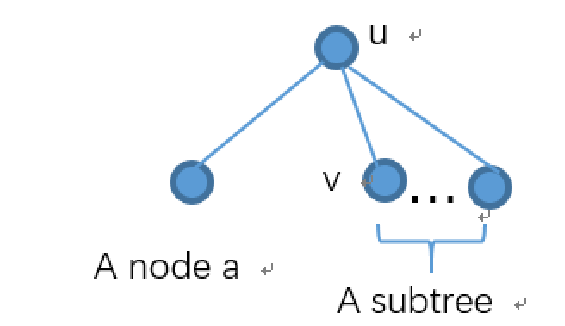
\includegraphics[width=0.7\linewidth]{hw2-1}
		\caption{34.2-11}
	\end{figure}
	\end{proof}
	\subsection*{32.3-2}
	\begin{proof}
		Suppose that $A_3$ is a polynomial-time algorithm for decision problem $L_3$, $F$ is a polynomial-time algorithm that calculates the reduction function $f$. Alike Figure 34-5 in the textbook, we can easily construct a polynomial-time algorithm $A_2$ for $L_2$. In the same way, we can also construct a polynomial-time algorithm $A_1$ from $A_2$ with the help of another reduction algorithm $F'$ and the function $f'$. The overall time complexity is still polynomial. Therefore, \[
		\left(L_1\le _PL_2\right)\land\left( L_2\le _PL_3\right)\implies\left(L_1\le _PL_3\right),
		\]
		i.e., the $\le_P$ relation is transitive.
	\end{proof}
	\subsection*{34.4-3}
	\begin{proof}
		The formula could have $O(n)$ free variables, therefore, the truth table corresponding to it would a number of rows that is $O(2^n)$ since it needs to
		consider every possible assignment to all the variables. This means that
		the reduction as described is going to increase the size of such problem exponentially. Consequently, it can not yield a polynomial-time reduction.

	\end{proof}
	\subsection*{34.4-5}
	\begin{proof}
		Denote the disjunctive formula by $\lor_i \phi_i$, where each $\phi_i$ represents $v_1\land v_2\land \cdots v_k$ ($v_i$ is either a variable or its negation). For each $\phi_i$, we examine whether it has some variable and its negation, if so, then the formula is not satisfiable. Otherwise, it can be satisfied. The total running time of this process is in $O(n)$, where $n$ is the size of all variables and/or its negations in the formula. Therefore, we prove that this problem is solvable in polynomial-time.
	\end{proof}
	\subsection*{34.4-7}
	\begin{proof}
		Suppose that the original formula was $\land_i(x_i \lor y_i)$, and the set of variables were
		${v_i}$. Then, consider the directed graph which has a vertex corresponding both
		to each variable, and its negation. Then, for each of the clauses
		$x\lor y$, place an edge from $\neg x$ to $y$, and an edge from $\neg y$ to $x$.
		Anytime an edge in the directed graph means that the vertex
		it originates is true, the vertex it points to should be true.
		Therefore, what we need to check is whether there exists a path from a vertex to its negation, or vice versa. If so, the formula is unsatisfiable. If not, then it is. In order to do this in a graph, we can run \proc{Strongly-Connected-Component} (The time complexity is $O(n)$) on the constructed graph. If any strongly-connected component contains both a variable $v_i$ and $\neg v_i$. Then return false, otherwise, return yes. In this way, we solve this problem in polynomial time. Therefore, $\text{2-CNF-SAT}\in\text{P}$
	\end{proof}
	\subsection*{34.5-6}
	%Ham path and Ham cycle, 一个是圈另一个是路径
	\begin{proof}
		In Exercise 34.2-6, it has been proved that \proc{Ham Path} belongs to NP. Denote language \proc{Ham Path} by $L$, we shall prove that
		$$\forall L'\in\text{NP},L'\le_P L.$$  
		To do this, we can prove that \proc{Ham Cycle}$\le_P$\proc{Ham Path}, since the former problem shown to be NP-complete.\\
		Let $G = (V, E)$ be any graph. We will construct a graph
		$G'$ as follows. For each edge $e_i \in G.E$, let $G_{e_i}$ denote the graph with vertex set
		$G.V$ and edge set $G.E − {e_i}$. Let $e_i$ have the form $\{u_i, v_i\}$. Now, $G'$ will contain one copy of $G_{e_i}$
		for each $e_i\in G.E$. Additionally, $G'$ will contain a vertex $x$ connected
		to $u_1$, an edge from $v_i to u_{i+1}$ for $1 \le i \le |G.E| − 1$, and a vertex $y$ and edge from
		$v_|G.E|$ to $y$. It is clear that we can construct $G'$
		from $G$ in polynomial time with regard to the
		size of $G$. Therefore, $\proc{Ham Cycle}\le_P \proc{Ham Path}$, \proc{Ham Path} is NP-complete.
	\end{proof}
	\subsection*{Exercise 2.3.3.8 (Revised)}
	\begin{enumerate}[(i)]
		\item A: Input: $(x,c)\in \left\{
		0,1,\sharp\right\}^\star\times \Sigma^\star_{bool}$
		\begin{enumerate}[(1)]
			\item 
			$x$ is a representation of a graph and we represent the set of vertices as $\left\{x_1,x_2,\dots,x_n\right\}$. $c$ codes a sequence of vertices: $I=\left\{x_{i1},x_{i2},\dots,x_{in},x_{i1}\right\}$.
			\item  If each pair of adjacent vertices have an edge, then A accepts $(x,c)$ otherwise A rejects it. 
		\end{enumerate}
		\item 
		A: Input: $(x,c)\in \{0,1,\sharp\}^+\times \Sigma_{bool}^{\star}$
		\begin{enumerate}[(1)]
			\item 
			$x=u\sharp w\in\{0,1,\sharp\}^+$ where $u\in\{0,1\}^+$ and $w$ represents a graph with $n$ vertices. Let $k=Number(u)$. $c\in \Sigma_{bool}^n$ codes $k$ vertices using $k$ symbols of 1.
			\item 
			If each edge of the graph is incident to at least one vertex in $c$, then A accepts $(x,c)$, otherwise, A rejects it. 
		\end{enumerate}
		\item 
		A: Input: $(x,c)\in\{0,1,\sharp\}\times \Sigma_{bool}^\star$
		\begin{enumerate}[(1)]
			\item 
			$x=u\sharp w\in\{0,1,\sharp\}^+$ where $u\in\{0,1\}^\star$ and $w$ represents a graph. Let $k=Number(u)$. $c$ codes $k$ vertices.
			\item 
			If each pair of the $k$ vertices has an edge, then A accepts $(x,c)$, otherwise, A rejects. 
		\end{enumerate}
	\end{enumerate}
\end{document}